\documentclass{article}
\usepackage[utf8]{inputenc}
\usepackage{amsmath}
\usepackage{hyperref}
\usepackage[pdftex]{graphicx}

%\usepackage{geometry}
\usepackage{wrapfig}
\usepackage{changepage}

\newcommand{\HRule}{\rule{\linewidth}{0.5mm}}
\newcommand{\tab}[1]{\hspace{.2\textwidth}\rlap{#1}}

\begin{document}
\begin{titlepage}
	\begin{center}
		
\includegraphics[width=0.30\textwidth]{Logo_UTFSM.png}~\\[1cm]
		\textsc{\LARGE Universidad Técnica Federico Santa María.}\\[1.2cm]
		\textsc{\Large Sistemas de Gestión.}\\[0.2cm]
		\textsc{\Large Departamento de Informática.}\\[0.2cm]
	
		% Title
		\HRule \\[0.4cm]
		{ \huge \bfseries La estrategia de Jobs en la Sociedad de Debate.\\[0.4cm] }
		\HRule \\[1.5cm]
		
		% Author and supervisor
		\begin{minipage}{0.9\textwidth}
			\large
			\emph{Resumen:} \\
			A once años de su creación, la Sociedad de Debate USM, debe
			enfrentar el reciente cambio de capitán. Por ello se analizaran aspectos
			relevantes de la gestión estratégica de Steve Jobs y como aplicarlos
			a la problemática de la Sociedad de Debate.
			\begin{flushright} 
				\emph{Palabras clave:} Debate, Estrategia, Steve Jobs.
			\end{flushright}
		\end{minipage}
		\vfill
	
		% Bottom of the page
		{\large Hernán Vargas Leighton.\\
		\href{mailto:hernan.vargas@alumnos.usm.cl}{hernan.vargas@alumnos.usm.cl}
		\\[0.2cm] \today }
	\end{center}
\end{titlepage}

\begin{adjustwidth}{-1.5cm}{-1.5cm}
	\section*{Sociedad de Debate.}
	La Sociedad de Debate de la Universidad Técnica Federico Santa María es una 
	organización nacida por la iniciativa de alumnos para mejorar las habilidades
	blandas, incentivar el intercambio de opiniones y representar a la institución
	en competencias deportivas de ésta disciplina. Todo comienza en el año 2003 cuando
	los miembros fundadores\footnote{Se han omitido los nombres intencionalmente} 
	deciden crear un equipo para representar nuestra institución
	en los torneos universitarios de debate, que en ese momento recién estaban
	comenzando en el país. El grupo, impulsado solo por el entusiasmo de los
	miembros, no logra ganar la tan ansiada copa, pero descubre un impensado
	interés en el debate por parte de algunos sansanos.\\[0.15cm]
	Con el paso del tiempo, la sociedad de Debate USM, pasa de ser un grupo de
	amigos que se reúne en el bloque libre para discutir temas de contingencia,
	a una sociedad con más de diez miembros regulares, docenas de asistentes al
	``Taller de Oratoria y Debate''\footnote{El ``Taller de Oratoria y Debate'' 
	es una iniciativa dirigida a alumnos de primer año de todas las carreras con
	el fin de mejorar las habilidades blandas y aprender los principios básicos
	del debate competitivo. Se realiza en el primer semestre de todos los años.}
	y participación constante en los más importantes torneos a nivel 
	local\cite{local}, nacional\cite{nac} e internacional\cite{inter}.\\[0.15cm]
	\begin{minipage}{0.7\textwidth}
		Actualmente la sociedad de debate se encuentra en un periodo de transición
		entre capitanes. Con la salida de quien fuera capitán por más de cuatro años,
		uno de los periodos de máximo crecimiento de la sociedad, el nuevo capitán
		se enfrenta al desafío de liderar un equipo ya maduro, compuesto tanto
		por miembros experimentados como por compañeros en proceso de aprendizaje
		y experimentación.\\
		Además está en las manos del nuevo capitán continuar con el Torneo Interescolar
		de Debate USM\cite{nac}, que esté año celebra su onceava edición. Además
		es su responsabilidad determinar la estrategia a seguir en los siguientes
		años para incrementar la cantidad de miembros del equipo, mantener el éxito
		de los talleres, obtener resultados en los torneos y aumentar el alcance
		de la sociedad tanto fuera como dentro de la universidad.
	\end{minipage}
	\hfill
	\begin{minipage}{0.5\textwidth}
		\begin{center}
			
\includegraphics[width=0.8\textwidth]{logo_debate.png}
		\end{center}
		Un nuevo logo\cite{logo} para la sociedad de debate es uno de los
		cambios sugeridos por la nueva capitanía.
	\end{minipage}

	\section*{Steve Jobs como estratega.}
	\begin{minipage}{0.35\textwidth}
		\begin{center}
			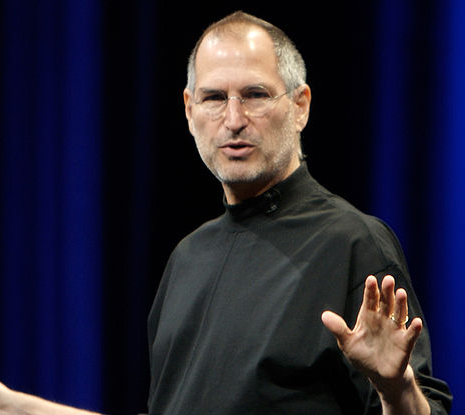
\includegraphics[width=0.85\textwidth]{jobs.png}
		Steve Jobs, 1955 - 2011.\\Fotografía de Acaben\cite{img}.
		\end{center}
	\end{minipage}
	\hfill
	\begin{minipage}{0.88\textwidth}
		El articulo ``Steve Jobs como estratega'' nos muestra algunas características
		por las cuales se llega a considerar a Jobs como uno de los más grandes
		estrategas de negocios de nuestra era. Se nos habla desde tres puntos:
		\begin{enumerate}
			\item[1.]
				\textbf{Inventor de Industrias:} El ingenio e iniciativa de Jobs
				le permitió sortear el ambiente desfavorable en el cual Apple se
				encontraba y crear una nueva industria, fortalecerla y hacer de
				ella una fuente de dinero para su compañía.
		\end{enumerate}
	\end{minipage}
	\begin{enumerate}
		\item[2.]
			\textbf{Intensamente Coherente:} La estrategia se basó en crear servicios
			y dispositivos compatibles entre si, de esta forma el usuario comenzaba
			con uno de sus dispositivos, como el iPhone, y gracias a la fácil 
			sincronización y compatibilidad terminaba utilizando todos sus servicios
			y comprando más de sus productos.
		\item[3.]
			\textbf{Creador de Empresas:} Jobs incentivaba el debate entre los 
			directivos de Apple, era muy honesto y  buscaba que todos los miembros
			trabajaran juntos para lograr los objetivos de la empresa.
	\end{enumerate}

	\section*{La estrategia de Jobs en la Sociedad de Debate.}
	Debido a las características de una iniciativa estudiantil, donde la competencia
	solo prima en la generación de interés y no se buscan resultados económicos,
	solo podemos aplicar la estrategia de Jobs en los puntos de coherencia y labor
	directiva.\\
	El ingreso de nuevos miembros es una de las principales preocupaciones de la
	sociedad para lograr mantenerse en el tiempo. La estrategia tomada por el
	capitán en este sentido será fundamental para la supervivencia de la organización,
	por ello, podemos basar nuestra estrategia en la coherencia como hizo Jobs.
	Los miembros que pasan a formar parte del equipo generalmente asisten
	al taller en primer lugar, pero no son un gran porcentaje de éste. Se podría
	ligar más la actividad de debate competitivo al taller de oratoria, para, de
	está manera, hacer que los miembros de está ultima permanezcan en la sociedad.\\
	Con respecto a la toma de decisiones, la Sociedad de Debate tiene un
	funcionamiento bastante parecido a lo que Jobs incentivaba en Apple, es decir:
	se fomenta la discusión, se habla con franqueza y se trabaja en equipo para
	el logro de los objetivos. 
	En general, podemos aprender de Jobs a no tener miedo a hacer cosas que nunca
	antes se han hecho, intentar ligarlas directa o indirectamente a la practica
	del debate competitivo y trabajar como un equipo dispuesto a discutir para
	lograr posicionarnos como una organización de prestigio dentro de la universidad.
	\begin{center}
		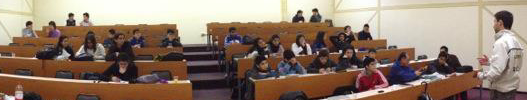
\includegraphics[width=0.8\textwidth]{sala.png}\\
		Taller de Debate USM. Fotografía propiedad de la Sociedad de Debate USM
	\end{center}

	\begin{thebibliography}{x}
		\bibitem{local}
			\href{http://www.comunicaciones.usm.cl/2011/07/08/sansanos-clasifican-a-semifinales-de-la-liga-de-debate-de-la-region/}
			{\textit{Sansanos clasifican a semifinales de la Liga de Debate de
			la Región}} - Dirección general de comunicaciones USM. Revisado el
			20 de Agosto del 2014.
		\bibitem{nac}
			\href{http://www.comunicaciones.usm.cl/2012/08/29/continua-exitoso-torneo-interescolar-de-debate-usm/}
			{\textit{Continúa exitoso Torneo Interescolar de Debate USM}} -
			Dirección general de comunicaciones USM. Revisado el 20 de Agosto del 2014.
		\bibitem{inter}
			\href{http://www.dgc.usm.cl/2013/03/21/usm-obtiene-tercer-lugar-en-torneo-de-debate-interuniversitario-2013-todi/}
			{\textit{USM obtiene tercer lugar en Torneo de Debate Interuniversitario
			2013 (ToDI)}} - Dirección general de comunicaciones USM. Revisado el
			20 de Agosto del 2014.
		\bibitem{logo}
			\textit{Logo Sociedad de Debate USM} - Creado por Fasny para la
			sociedad de debate USM.
		\bibitem{img}
			\href{http://www.flickr.com/photos/acaben/541420967/in/set-72157603723478753/}
			{\textit{Steve Jobs keynote}} - Flickr. Revisado el 20 de Agosto del 2014.
\vfill\hfill Tiempo SCT: 7:38 / \LaTeXe
	\end{thebibliography}
\end{adjustwidth}

\end{document}
